\documentclass[12pt, titlepage, letterpaper]{article}
%\documentclass[12pt, letterpaper, titlepage]{article}

\usepackage{amsmath}
\usepackage{booktabs}
\usepackage{amsthm}
\usepackage{graphicx}
\usepackage[margin=1in]{geometry}
\usepackage{hyperref}
\hypersetup{colorlinks = true, linkcolor = blue, citecolor=blue, urlcolor = blue}
\usepackage{natbib}
\usepackage{enumitem}
\usepackage{setspace}


\usepackage[]{lineno}
\linenumbers*[1]
% %% patches to make lineno work better with amsmath
\newcommand*\patchAmsMathEnvironmentForLineno[1]{%
 \expandafter\let\csname old#1\expandafter\endcsname\csname #1\endcsname
 \expandafter\let\csname oldend#1\expandafter\endcsname\csname end#1\endcsname
 \renewenvironment{#1}%
 {\linenomath\csname old#1\endcsname}%
 {\csname oldend#1\endcsname\endlinenomath}}%
\newcommand*\patchBothAmsMathEnvironmentsForLineno[1]{%
 \patchAmsMathEnvironmentForLineno{#1}%
 \patchAmsMathEnvironmentForLineno{#1*}}%

\AtBeginDocument{%
 \patchBothAmsMathEnvironmentsForLineno{equation}%
 \patchBothAmsMathEnvironmentsForLineno{align}%
 \patchBothAmsMathEnvironmentsForLineno{flalign}%
 \patchBothAmsMathEnvironmentsForLineno{alignat}%
 \patchBothAmsMathEnvironmentsForLineno{gather}%
 \patchBothAmsMathEnvironmentsForLineno{multline}%
}

% control floats
\renewcommand\floatpagefraction{.9}
\renewcommand\topfraction{.9}
\renewcommand\bottomfraction{.9}
\renewcommand\textfraction{.1}
\setcounter{totalnumber}{50}
\setcounter{topnumber}{50}
\setcounter{bottomnumber}{50}

\newcommand{\jy}[1]{\textcolor{blue}{JY: #1}}
\newcommand{\eds}[1]{\textcolor{red}{EDS: (#1)}}
\newcommand{\mc}[1]{\textcolor{green}{MC: (#1)}}

% NOTE: To produce blinded version, replace "0" with "1" below.
\newcommand{\blind}{1]}

\begin{document}
%\maketitle

\title{Nonparametric Block Bootstrap Kolmogorov-Smirnov Goodness-of-Fit Test}
\if0\blind
{
  \author{Mathew Chandy, %\\
%   \href{mailto:mathew.chandy@uconn.edu}
%   {\nolinkurl{mathew.chandy@uconn.edu}}\\
  Elizabeth Schifano\\
  Jun Yan\\
  Xianyang Zhang\\
} \fi


\maketitle


\begin{abstract}

The Kolmogorov-Smirnov (KS) test is a widely used statistical test that
assesses the conformity of a sample to a specified distribution. Its efficacy,
however, diminishes with serially dependent data and when parameters
within the hypothesized distribution are unknown. For independent data,
parametric and nonparametric bootstrap procedure are available to adjust for
estimated parameters. For serially dependent stationary data, parametric
bootstrap has been developed with a working serial dependence structure. A
counterpart for the nonparametric bootstrap approach, which needs a bias
correction, has not been studied. Addressing this gap, our study introduces a
bias correction method employing a non-parametric block bootstrap, which
adeptly the distribution of the KS statistic for by unspecified serial
dependence and unspecified parameters. We assess its effectiveness
through simulations, scrutinizing both its size and power. The practicality of
our method is further illustrated with an examination of stock returns from the
S\&P 100 and S\&P 500 indices, showcasing its utility in real-world
applications.

\bigskip
\noindent{\sc Keywords}:
bias-correction; 
serial dependence;
time series. 
\end{abstract}

\doublespace 


\section{Introduction}
\label{sec:intro}

The standard one-sample Kolmogorov-Smirnov (KS) test is widely
recognized as an effective good-of-fit test for continuous distributions.
Consider $X_1, ..., X_n$, a random sample of size~$n$ from some continuous
distribution and the null hypothesis $H_0$ that $X_i$'s follow a specific
hypothesized distribution~$F$.
If we let $F_n(t) = \sum_{i=1}^n I(X_i \le t) / n$ be the empirical cumulative
distribution function of the sample, where $I(\cdot)$ is the indicator
function, the KS test statistic takes the form
\begin{equation}
  \label{eq:ks_standard}
  T_n = \sqrt{n} \sup_x | F_{n}(x) - F(x) |.
\end{equation}
As sample size $n\to \infty$, the distribution of $T_n$ converges to that of the
absolute value of standard Brownian bridge, which is known as the Kolmogorov
distribution \citep{stephens1974edf}. This distribution function is
precisely computable using contemporary statistical software
\citep{marsaglia2003evaluating}. The versatility of the KS test allows its
application across various domains, such as analyzing cosmic microwave
background radiation \citep{naess2012application}, monitoring the count rate of
radioactive data \citep{aslam2020introducing}, gear condition monitoring
\citep{andrade2001gear}, studying images of breast cancer tumors
\citep{demidenko2004kolmogorov}, and examining financial markets
\citep{lux2001turbulence}.


Despite its widespread use, the KS test can be 
misapplied when its foundational assumptions are overlooked. The KS test 
assumes the data are independently and identically distributed (i.i.d.) and 
\jy{no defining acronyms that are not used later}
that the hypothesized distribution is continuous and fully specified without 
the need for parameter estimation. \citet{zeimbekakis2022misuses} examines
common misapplications of the one-sample KS test. One notable inappropriate
use is when the hypothesized distribution contains unspecified parameters.
In this case, the tests are generally constructed by substituting the unknown
parameters by their estimates, and the asymptotic null distribution of
the test statistic may depend in a complex way on the unknown parameters.
The problem of unspecified parameters can be handled by a parametric
bootstrap, where bootstrap samples of the test statistics are constructed from
samples generated from the fitted hypothesized distribution.
Alternatively, \citet{babu2004goodness} address this issue through a
non-parametric bootstrap method that corrects the bias in the asymptotic null
distribution.



Another prevalent misapplication of the KS test arises when data exhibit serial
dependence, which is often overlooked in analyses. For example, in an
investigation of performance variation in high-performance computing systems,
\citet{tuncer2019ieee} did not describe how or if they accounted for serial
dependence when applying the two-sample KS test.
\citet{zeimbekakis2022misuses} proposed a semi-parametric bootstrap
where the serial dependence structure is modeled via a working serial copula.
A particularly complex scenario arises when the distribution has unspecified
parameters, and the data are serially dependent. For this,
\citet{zeimbekakis2022misuses} also recommends a semi-parametric bootstrap
approach, where the parameters of the hypothesized distribution and the serial
dependence both need to be estimated and their uncertainty accounted for.


Developing a fully non-parametric solution for the KS 
tests in the presence of serially dependent data presents a significant 
challenge. The null distribution's characteristics are intricately linked to 
the structure of the serial dependence, which can vary widely in practical 
situations. Employing a non-parametric bootstrap would necessitate defining a 
specific model for this dependence, despite the primary focus being on 
evaluating the marginal distribution of a stationary series. To date, a bias 
correction method for block bootstrap, akin to the non-parametric bootstrap
approach of \citet{babu2004goodness} for independent data,
has not been established. This study seeks 
to bridge this gap by introducing a bias correction technique for the 
non-parametric block bootstrap, tailored for use in scenarios where the 
hypothesized distribution includes unspecified parameters and the data 
exhibit serial dependence. Our approach reduces to that of
\citet{babu2004goodness} when the data are independent.


The remainder of this paper is structured as follows: 
Section~\ref{sec:methods} provides an overview of the block bootstrap 
procedure and introduces the bias correction methodology for the 
non-parametric block bootstrap KS test. Section~\ref{sec:simu} is divided 
into two parts; initially, we evaluate the KS test's ability to maintain 
its size, i.e., its consistency in not rejecting the null hypothesis when 
it is indeed true. Subsequently, we examine the test's power, assessing 
whether it can reject the null hypothesis when it is false. Practical 
applications of our method are presented in Section~\ref{sec:real}, where 
we apply the approach to analyze if S\&P 100 and S\&P 500 index stock return
data adhere to either the Normal or the Student's $t$ distribution. The 
paper concludes with Section~\ref{sec:conclusion}, offering final thoughts 
and remarks.


\section{Methods}
\label{sec:methods}

Consider a stationary time series $\{X_t: t = 1, \ldots, n\}$ with length~$n$.
We are interested in testing whether or not $X_t$ follows a distribution in a
parametric family of distribution~$F$ indexed by a parameter
vector~$\theta$. That is, the null hypothesis is
\[
  H_0: X_t \sim F(\cdot \mid \theta), \quad t = 1, \ldots, n,
\]
for some unspecified parameter $\theta$.
The alternative hypothesis $H_A$ is that the marginal distribution of $X_t$ does
not follow~$F$ for any parameter value~$\theta$. This is a challenging situation
because both the parameters and the serial dependence structure are unknown.

\subsection{Kolmogorov--Smirnov Test}

First, let us review how the KS statistic is typically computed for a sample
with no serial dependence with fitted parameters.
Let $\hat\theta_n$ denote the fitted parameters for the hypothesized 
distribution fitted onto $X_t$, and let 
$F_n$ denote the empirical distribution function based on $X_1,...,X_n$.
Let
\begin{equation*}
Y_n(x; \hat\theta) = \sqrt{n}(F_n(x) - F(x; \hat\theta_n)).
\end{equation*}
Then, the
goodness of fit statistic is 
\begin{equation*}
T_n := \sup_x|Y_n(x; \hat\theta)|.
\end{equation*}

\jy{State clearly the test statistic definition. Point out that the null
  distribution depends on the unknown parameters and unknown serial
  dependence. Point out the challenges are to approximate the null distribution.}

We note that
\begin{equation*}
Y_n(x; \hat\theta) = \sqrt{n}(F_n(x) - F(x)) - 
\sqrt{n}(F(x; \hat\theta_n) - F(x)),
\end{equation*}
\jy{clean up the notations. Has $F$ been defined yet? do you need cdf?}
where $F(x)$ is the true cdf (under the null $F(x) = F(x, \theta_0)$ for some
true parameter $\theta_0$).

\subsection{Non-Parametric Bootstrap for Independent Data}

Let us then consider the case where $X_i$'s are independent, but parameters
are unspecified. Denote by
$F^{(b)}_n$ the empirical distribution of the $b$th bootstrap sample and let
$\hat\theta^{(b)}_n$ be the parameter estimate based on the $b$th bootstrap 
sample. 
Using the bootstrap (asymptotic) theory, we can approximate the distribution of
$\sqrt{n}(F_n(x) - F(x))$ and $\sqrt{n}(F(x; \hat\theta_n) - F(x))$
by that of $\sqrt{n}(F^{(b)}_n(x) - F_n(x))$ and
$\sqrt{n}(F(x; \hat\theta^{(b)}_n) - F(x; \hat\theta_n))$, respectively.
Therefore, if we define
\begin{align*}
Y^{(b)}_n(x) &= \sqrt{n}(F^{(b)}_n(x) - F_n(x)) - 
               \sqrt{n}(F(x; \hat\theta^{(b)}_n) - F(x; \hat\theta_n)) \\
             &= \sqrt{n}(F^{(b)}_n(x) - F(x; \hat\theta^{(b)}_n)) - 
               \sqrt{n}(F_n(x) - F(x; \hat\theta_n)),
\end{align*}
then $T^{(b)}_n := \sup_x|Y^{(b)}_n(x)|$ is the bootstrap statistic that is 
expected to approximate the distribution of $T_n$. We note that the term
$\sqrt{n}(F_n(x) - F(x; \hat\theta_n))$ is exactly the bias term considered in 
\citet{babu2004goodness}.

In summary, the procedure of the nonparametric basic bootstrap test is 
summarized as follows. Repeat the following steps for $b \in \{1, ..., B\}$.
\begin{enumerate}
\item
  Generate $X^{(b)}_1,...,X^{(b)}_n$ by applying basic bootstrap 
  on the original sample as
  defined previously.
\item
  Fit $F_\theta$ to $X^{(b)}_1,...,X^{(b)}_n$ and obtain estimate 
	$\hat\theta^{(b)}_n$ of $\theta$.
\item
  Obtain the empirical distribution function $F^{(b)}_n$ of
  $X^{(b)}_1,...,X^{(b)}_n$. 
\item
  Calculate bootstrap KS statistic
  \[
    T^{(b)}_n = \sup_x | \sqrt{n}\left(F^{(b)}_n(x) 
    - F(x; \hat\theta^{(b)}_n)\right) - B_n(x) |.
  \]
  where 
  $B_{n}(x) = \sqrt{n}(F_n(x) - F(x; \hat\theta_n))$ is the known
  bias term.
\end{enumerate}


The p-value of the basic bootstrap KS test can be approximated
as $p = \sum_{b=1}^BB I\{T^{(b)}_n > T_n\} / B$.

\subsection{Non-Parametric Block Bootstrap for Stationary Series}

We now consider the case where $X_i$'s are realizations from a time series and
$X^{(b)}_1,...,X^{(b)}_n$ are generated by block bootstrap for 
$b \in \{1, \ldots, B\}$.  
Block-bootstrap can be done with overlapping or moving blocks.
Define moving blocks (assuming $l > 1$) as:
\begin{equation*}
Z_j =
    \begin{cases}
        \{X_j, \ldots, X_{j + l - 1}\}, & j = 1, \dots, n - l + 1,\\
        \{X_j, \ldots, X_n, X_1, \ldots, X_{j-n+l-1}\}, & j = n - l
        + 2 ,\dots, n.
    \end{cases}
\end{equation*}
A common 
function for block size that is considered optimal is 
$l = \lceil n^{1/3} \rceil$ \citep{buhlmann1999block},  
which was adopted in this study.
Now we draw $k$ blocks from the $(n - l + 1)$ blocks 
of $Z_j$'s with replacement and then align them in the order they were picked to
form a block bootstrap sample. If $n$ is not a multiple of~$l$, the last block 
selected will be reduced in size so that the final size of the block bootstrap 
sample is $n$.


Continuing using the notation in the independent case,
we use $F^{(b)}_n$ and $\hat\theta^{(b)}_n$ for the empirical distribution and
the estimated parameters based on the $b$th bootstrap sample,
$b = 1, \ldots, B$.
We then use block bootstrap to approximate the asymptotic distribution of
the KS statistic under $H_0$. In particular, we
use the distribution of $\sqrt{n}(F^{(b)}_n(x) - E[F^{(b)}_n(x)])$
as an approximation of the distribution of
$\sqrt{n}(F_n(x) - F(x))$, and the distribution of 
$\sqrt{n}(F(x; \hat\theta^{(b)}_n) - F(x; E[\hat\theta^{(b)}_n]))$ as
an approximation of the distribution of $\sqrt{n}(F(x; \theta_n) - F(x))$.
The expected values $E[F^{(b)}_n(x)]$ and
$E[\hat\theta^{(b)}_n]$ can be approximated by, respectively,
$E_n[F^{(b)}_n(x)] = \frac{1}{B}\sum_{b = 1}^BF^{(b)}_n(x)$ and
$E_n[\hat\theta^{(b)}_n]  =  \frac{1}{B}\sum_{b = 1}^B\hat\theta^{(b)}_n$.


Then, we can define
\begin{align*}
  Y^{(b)}_n(x) &= \sqrt{n}(F^{(b)}_n(x) - E[F^{(b)}_n(x)]) - 
             \sqrt{n}(F(x; \hat\theta^{(b)}_n) - F(x; E[\hat\theta^{(b)}_n)]) \\
           &= \sqrt{n}(F^{(b)}_n(x) - F(x; \hat\theta^{(b)}_n)) -
             \sqrt{n}(E[F^{(b)}_n(x)] - F(x; E[\hat\theta^{(b)}_n])),
\end{align*}
and $T^{(b)}_n = \sup_x|Y^{(b)}_n(x)|$. Each $T_n^{(b)}$,
$b =1, \ldots, B$, is considered a draw from a distribution that approximates
the distribution of $T_n$. Therefore, the p-value of the observed statistic
$T_n$ can be assessed by positioning it agains the empirical distribution of
$T_n^{(b)}$, $b = 1, \ldots, B$.


In summary, the procedure of the nonparametric block bootstrap test is 
summarized as follows. Repeat the following steps for $b \in \{1, ..., B\}$.
\begin{enumerate}
\item
  Generate $X^{(b)}_1,...,X^{(b)}_n$ by applying moving block bootstrap 
  on the original sample as
  defined previously.
\item
  Fit $F_\theta$ to $X^{(b)}_1,...,X^{(b)}_n$ and obtain estimate 
	$\hat\theta^{(b)}_n$ of $\theta$.
\item
  Obtain the empirical distribution function $F^{(b)}_n$ of
  $X^{(b)}_1,...,X^{(b)}_n$. 
\item
  Calculate bootstrap KS statistic
  \[
    T^{(b)}_n = \sup_x | \sqrt{n}\left(F^{(b)}_n(x) 
    - F(x; \hat\theta^{(b)}_n)\right) - B_n(x) |.
  \]
  where 
  $B_{n}(x) = \sqrt{n}(E[F^{(b)}_n(x)] - 
  F(x; E[\hat\theta^{(b)}_n]))$ is the known
  bias term.
\end{enumerate}


The p-value of the block bootstrap KS test can be approximated
as $p = \sum_{b=1}^N I\{T^{(b)}_n > T_n\} / B$.


\section{Simulation Studies}
\label{sec:simu}

In this simulation study, our objective is twofold: firstly, to demonstrate that
under the null distribution, our test rejects the null hypothesis ($H_0$) 
approximately at the specified significance level. Secondly, we aim to
illustrate that under the alternate distribution, our test reliably rejects
$H_0$ at a high frequency. The fulfillment of both these criteria would indicate
the method's efficacy.


\subsection{Size}
We first must evaluate whether this method works when $H_0$ is true. To
test this, we can
generate a simulated sample $X_t$ with a certain marginal distribution 
$F_\theta$,
and use our method to test if $X_t$ indeed has the marginal distribution $F$ 
with some unknown $\theta$. If the test holds its size, the 
p-value
of the test should be uniformly distributed between 0 and 1. We must try the
method with different marginal distributions to ensure that it is robust.
In order for the method to work, a large sample size may be necessary. 


We generated time series with marginal distributions $N(8, 8)$ and
$\Gamma(8, 1)$ with Kendall's
$\tau \in \{-.75, -.5, -.25, 0, .25, .5, 75\}$, and
sample size $n \in \{100, 200, 400, 800\}$. Kendall's $\tau$ was chosen as a
measure of serial dependence as it does not vary between two different 
marginal distributions.
To generate the samples to which our
method would be applied, we simulated a time series $W_t$ from a 1st 
order autoregressive (AR(1)) process:
\begin{equation*}
W_t = \phi X_{t-1} + \epsilon_t,
\end{equation*}
where $\phi$ is an autoregressive coefficient, and $\epsilon_t$ is a series of
independent errors from a normal distribution with mean zero and variance
$\sigma_{\epsilon}^2$. The strength of the serial dependence is controlled by
$\phi$, which was set to five levels: 
$\{-0.924, -0.707, -0.383, 0, 0.383, 0.707, 0.924\}$, as these
correspond to the desired values for $\tau$. First, we generated a
marginal $N(8, 8)$ by marginally transforming $W_t$ by
\begin{equation*}
X_t = F^{-1}[\Phi(W_t)],
\end{equation*}
\jy{define $\Phi$}
\jy{The language issues are more than I expected. Please do a careful proofread,
  now that you are more experienced.}
where $F^{-1}(p)$ is the quantile function for the $N(8, 8)$ 
distribution.
Then we generated a marginal gamma series by the same procedure, but
replacing $F^{-1}(p)$ with the quantile function for the $\Gamma(8, 1)$
distribution.
After the transformation
to the marginal gamma distribution, the autocorrelations are $\{-0.884, 
-0.686, -0.389, -0.033, 0.327, 0.639, 0.861\}$.


These distributions
were chosen to compare results on normal and non-normal
error structures. The specific parameters were chosen because the distributions 
are very similar and their
first two moments are the same. 
For the purposes of 
evaluating if the test holds it size, when $X_t \sim N(8, 8)$, we tested that the 
marginal distribution is from the
Normal family, or 
$X_t \sim N(\cdot \mid \mu, \sigma^2), \quad t = 1, \ldots, n$
for some unspecified $\mu$ and $\sigma$. When $X_t \sim \Gamma(8, 1)$, we tested
that the marginal distribution family is from the Gamma family,
or
$X_t \sim \Gamma(\cdot \mid \alpha, \beta), \quad t = 1, \ldots, n$.
for some unspecified $\alpha$ and $\beta$.
For the block
bootstrap step,
we used $B = 1000$ and $l = \lceil n^{1/3} \rceil$.
For each setting for $F$, $\tau$, and $n$, we replicate the method 1000 times 
to get the distribution of the p-values 
for the test when applied to samples from the same data generating process.


Using the \textsl{qqplotr} and \textsl{ggplot2} packages 
\citep{qqplotr, ggplot2},
we constructed Q-Q plots of the distribution of the p-values to see if they are
uniformly distributed. If the distribution of the p-values is uniform, this 
indicates that under the null hypothesis, our method will only reject the $H_0$
at a rate of $\alpha$.
A zoomed in plot for probabilities between 0 and 0.1 is
also provided, as
that is the most common range for significance levels $\alpha$. 
%We can also
%compute the rate of rejection $\#P < \alpha$ for different values of
%$\alpha$, as well as a confidence interval
%for this proportion.

\begin{figure}[tbp]
  \centering
  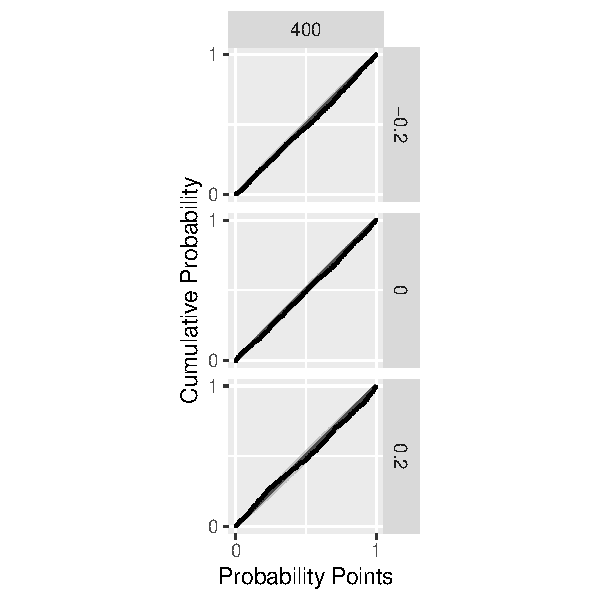
\includegraphics[width = \textwidth]{figures/normal}
  \caption{A Q-Q plot of the p-values testing that a distribution
  generated from a $N(8,8)$ data generating process is normal.}
  \label{fig:normal}
\end{figure}

\begin{figure}[tbp]
  \centering
  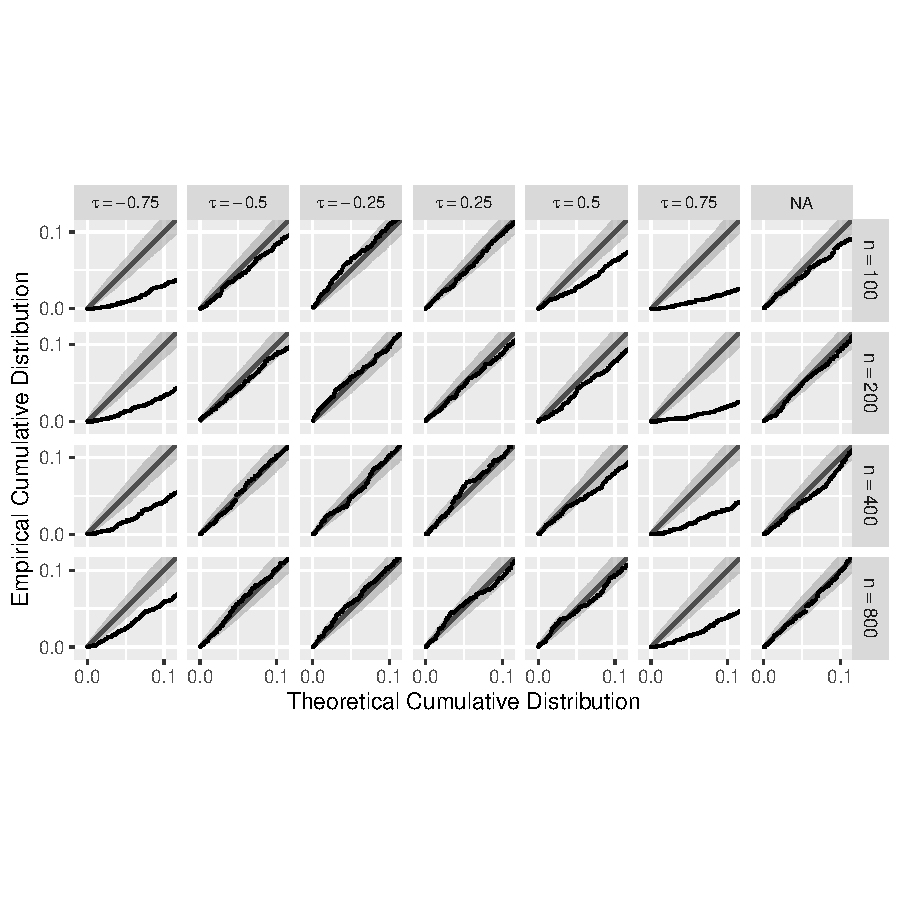
\includegraphics[width = \textwidth]{figures/zoom_normal}
  \caption{A Q-Q plot of the p-values displayed in Figure~\ref{fig:normal} zoomed in to 
  probabilities between 0 and
  0.1}
  \label{fig:zoom_normal}
\end{figure}

\begin{figure}[tbp]
  \centering
  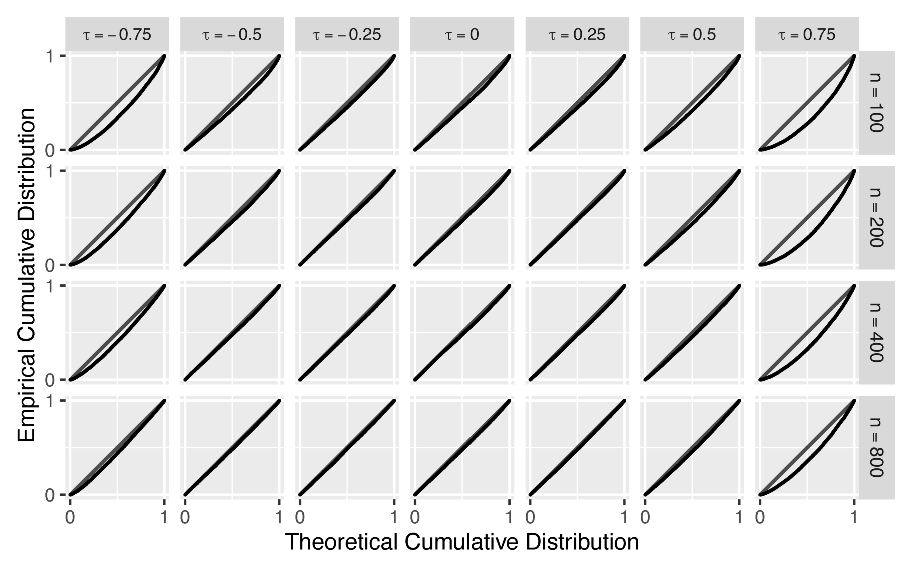
\includegraphics[scale=1]{figures/gamma}
  \caption{A Q-Q plot of the p-values testing that a distribution
  generated from a $\gamma(8,1)$ data generating process is gamma distributed.}
  \label{fig:gamma}
\end{figure}

\begin{figure}[tbp]
  \centering
  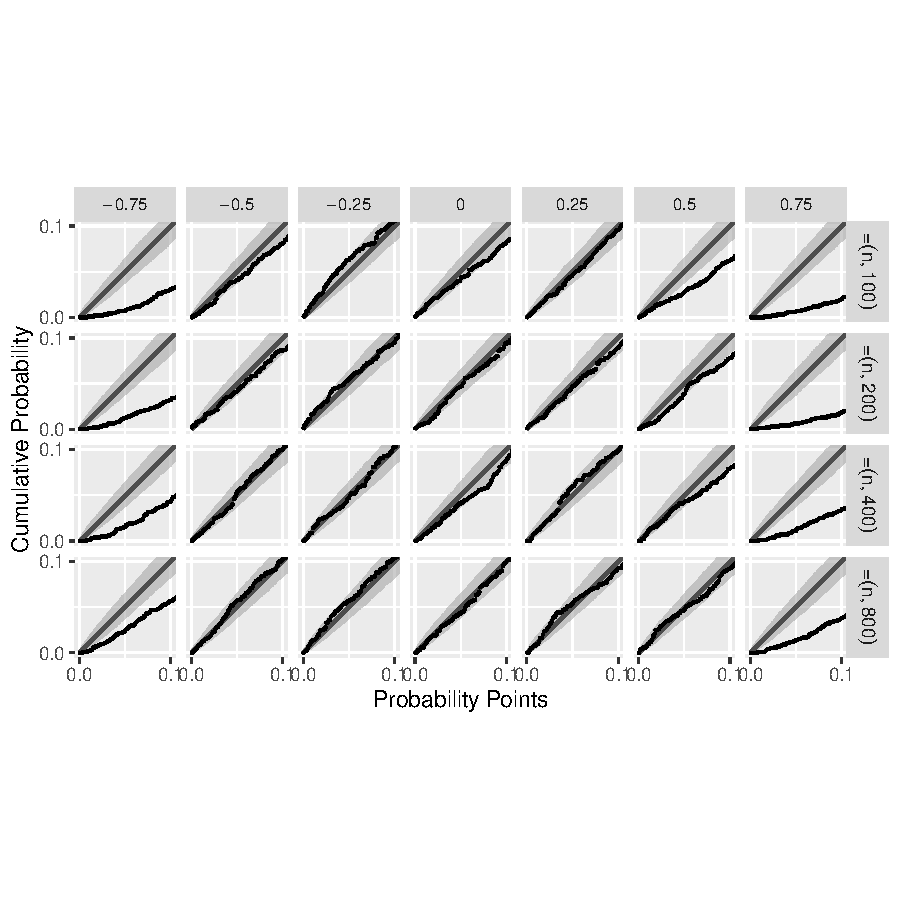
\includegraphics[scale=1]{figures/zoom_gamma}
  \caption{A Q-Q plot of the p-values displayed in Figure~\ref{fig:gamma} zoomed in to 
  probabilities between 0 and
  0.1}
  \label{fig:zoom_gamma}
\end{figure}

From Figures~\ref{fig:normal} and \ref{fig:gamma}, we can observe that 
although the extent to which the p-values appear to be 
completely aligned with the line
in the Q-Q plots is dependent on the sample size and the level of serial 
dependence.
A small sample size like $n = 100$ or $200$ seems adequate when Kendall's
$\tau$ is lower than 0.25. For Kendall's $\tau \geq 0.5$, a sample larger than
$n = 200$ seems necessary for the p-values to be normally distributed. For
Kendall's $\tau \geq 0.75$, a sample larger than $n = 800$ appears to be 
necessary, as the p-values are not aligned with the line in the Q-Q plots, even
in Figures~\ref{fig:zoom_normal} and \ref{fig:zoom_gamma}. This
is not necessarily a cause for concern, as (for normal margins)
a Kendall's $\tau$ corresponds to
a $\phi$ of 0.924, which is very high. Additionally, performance generally seems
better for negative $\tau$ values versus positive $\tau$ values of the same
strength. Results are very similar for normal and gamma margins.


Under $H_0$, the p-values for the non-parametric block bootstrap KS test are
uniformly distributed. This is an indication that our method 
holds its size and that we can expect the probability
of a type 1 error to be the significance level $\alpha$.


\subsection{Power}
We must also evaluate if this method works when $H_0$ is false. We can use
the block bootstrap KS test to test if some $X_t \sim F$ is generated from 
some other 
distribution $G$ with some unknown $\theta$. In this scenario, if the test is 
indeed powerful,
we would ideally want $\beta$ 
(or the probability of failed rejection under $H_A$) 
to be 0, but we
expect it to be generally low. Again, we must try the method with different
marginal distributions to ensure that it is robust.
We would then expect the distribution of p-values to be non-uniform, and the 
rate
of $\#P < \alpha$ to be high, meaning a higher density of low p-values.


Like we did to see if the test holds its size, we generated time series with 
marginal distributions $N(8, 8)$ and 
$\Gamma(8, 1)$, Kendall's $\tau \in \{-.75, -.5, -.25, 0, .25, .5, 
.75\}$, and
sample size $n \in \{100, 200, 400, 800\}$. However, 
to evaluate the test's power, when $X_t \sim N(8, 8)$, we tested
that the marginal distribution family is from the Gamma family,
or
$X_t \sim \Gamma(\cdot \mid \alpha, \beta), \quad t = 1, \ldots, n$.
for some unspecified $\alpha$ and $\beta$. Because the support of $N(8, 8)$ is
$(-\infty, \infty)$, but the support of $\Gamma(8, 1)$ is $(0, \infty)$, we used
the \textsl{truncdist} package \citep{truncdist} to truncate the series at 
values less than or equal to 0.
When $X_t \sim \Gamma(8, 1)$, we tested that the 
marginal distribution is from the
Normal family, or 
$X_t \sim N(\cdot \mid \mu, \sigma^2), \quad t = 1, \ldots, n$
for some unspecified $\mu$ and $\sigma$. For the block bootstrap step,
we used $B = 1000$ and $l = \lceil n^{1/3} \rceil$.
For each setting for $F$, $\tau$, and $n$, we replicate the method $1000$ times 
to obtain a p-value $p_r$ for each $r \in \{1, \ldots, 1000\}$.


Given some significance level $\alpha$, we can compute a rejection rate 
$q = \#\{p_r < \alpha\} / 1000$ for $r \in \{1, \ldots, 1000\}$.
Additionally, we can construct a 95\% confidence interval for 
this rate. Below are tables containing rejection rates showcasing the 
differences when simulation settings are changed.


\begin{figure}[tbp]
  \centering
  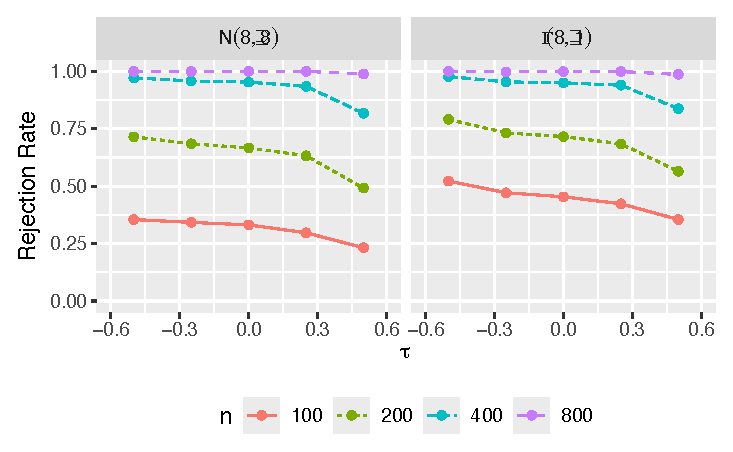
\includegraphics[scale=1]{figures/rr}
  \caption{A plot of the rejection rates as a function of $\tau$ for
 $n \in \{100, 200, 400, 800\}$ and marginal distribution 
 $\in \{N(8,8), \Gamma(8,1)\}$.}
  \label{fig:rr}
\end{figure}


From 
Figure~\ref{fig:rr}, 
the rejection rates appear to get lower as $\tau$ increases in a
positive direction. Using a sample size $n \geq 800$ appears to be sufficient
when $\tau$ is not too high, but for $\tau \geq 0.75$, all sample sizes 
observed appeared to have less than desirable rejection rates. Results
do not appear to be to different when comparing gamma and normal 
margins, indicating that the method is robust to the marginal distribution.
The rejection rates for $n = 800$ are very 
high (almost 1), indicating that under $H_A$, the test is very powerful 
(low probability of failed rejection $\beta$) when a large enough
sample size is used.


\section{Real Data Analysis}
\label{sec:real}

Using the \textsl{tseries} package 
\citep{tseries}, 
we gathered closing stock prices for the S\&P 500 index. We
observed how the method performs using the last 
4 years of data: January 1st, 2020 to December 31st, 2023.
We approximated stock returns by taking the difference in the logarithm 
of the closing prices.
Using our method, we tested that the stock returns are normally
distributed and Student's $t$ distributed 
with degrees of freedom $v \in \{30, 20, 10, 5, 4, 3, 2, 1\}$.
We tested the same hypotheses using \citet{babu2004goodness}'s 
non-parametric basic bootstrap bias correction and 
\citet{zeimbekakis2022misuses}'s parametric bootstrap method.
We used $B = 10,000$ bootstrap 
replicates in this analysis.
The p-values for these tests are highlighted in 
Table~\ref{table:SP5004}. 

Once again, utilizing the \textsl{tseries} package \citep{tseries}, we collected
closing stock prices for the S\&P 100 index. Employing the same methodology as
our study on the S\&P 500 index, we conducted our analysis. The resulting 
p-values for these tests are presented in Table~\ref{table:SP1004}.

% latex table generated in R 4.3.0 by xtable 1.8-4 package
% Fri Mar 15 20:41:15 2024
\begin{table}[ht]
\centering
\caption{P-values for 4 years of SP500 stock return 
                   data using different durations
  and different degrees of freedom for Student's t distribution.} 
\label{table:SP5004}
\begin{tabular}{rlllll}
  \hline
 & duration & df & block & basic & param \\ 
  \hline
1 & 4 & norm & 1e-04 & 0 & 0 \\ 
  2 & 4 & 30 & 0.0019 & 0 & 0 \\ 
  3 & 4 & 20 & 0.0027 & 0 & 0 \\ 
  4 & 4 & 10 & 0.0125 & 3e-04 & 3e-04 \\ 
  5 & 4 & 5 & 0.061 & 0.0222 & 0.0141 \\ 
  6 & 4 & 4 & 0.1037 & 0.0574 & 0.0499 \\ 
  7 & 4 & 3 & 0.3133 & 0.2759 & 0.2686 \\ 
  8 & 4 & 2 & 0.0418 & 0.0377 & 0.0443 \\ 
  9 & 4 & 1 & 0 & 0 & 0 \\ 
   \hline
\end{tabular}
\end{table}



% latex table generated in R 4.3.0 by xtable 1.8-4 package
% Mon Mar 11 20:21:19 2024
\begin{table}[ht]
\centering
\caption{P-values for 4 years of SP100 stock return 
                   data using different durations
  and different degrees of freedom for Student's t distribution.} 
\label{table:SP1004}
\begin{tabular}{rlllll}
  \hline
 & duration & df & block & basic & param \\ 
  \hline
1 & 4 & norm & 0.002 & 0 & 0 \\ 
  2 & 4 & 30 & 0.002 & 0 & 0 \\ 
  3 & 4 & 20 & 0.002 & 0 & 0 \\ 
  4 & 4 & 10 & 0.006 & 0 & 0 \\ 
  5 & 4 & 5 & 0.092 & 0.031 & 0.027 \\ 
  6 & 4 & 4 & 0.266 & 0.197 & 0.182 \\ 
  7 & 4 & 3 & 0.456 & 0.439 & 0.428 \\ 
  8 & 4 & 2 & 0.011 & 0.023 & 0.027 \\ 
  9 & 4 & 1 & 0 & 0 & 0 \\ 
   \hline
\end{tabular}
\end{table}



While differences in p-values among different methods are expected, our analysis
reveals numerous instances where conclusions at the 0.05 significance level
using our method differ from those obtained using the methods proposed by
\citet{babu2004goodness} and \citet{zeimbekakis2022misuses}.

For example, when assessing the S\&P 500 series, our method fails to reject the
hypothesis that the series follows a Student's $t$ distribution with degrees of
freedom $v = 5$ with a p-value of 0.061. In contrast, Babu and Sen's method
yields a p-value of 0.0222, and Zeimbekakis et al.'s method yields a p-value of
0.0141. Although such differences are not guaranteed, this
instance highlights a disagreement in conclusions among methods for the S\&P 500
index.

For the S\&P 100 index, our method demonstrates more instances where it reaches
different conclusions at the 0.05 significance level compared to other methods.
Our method fails to reject the hypothesis that the series conforms to a
Student's $t$ distribution with degrees of freedom $v = 5$, yielding a p-value
of 0.0873. In contrast, \citet{babu2004goodness}'s method yields a p-value of 
0.0368, and \citet{zeimbekakis2022misuses}'s method yields a p-value of 0.03. 
We have here
another instance where employing different methods leads to divergent
conclusions regarding the marginal distribution of the population under scrutin.


\section{Concluding Remarks}
\label{sec:conclusion}

The Kolmogorov-Smirnov test stands as a crucial tool for researchers across
diverse fields, enabling comparisons of population distributions. This paper
introduces a variant of the test tailored for serially dependent data without
necessitating parameter specification.
Using simulation, we have shown that given a large enough sample of a time 
series, the block 
bootstrap KS test can appropriately fail to reject the null hypothesis when the
series follows the null distribution. In addition, when the marginal
distribution is not
the one hypothesized, the test is powerful. Notably, it demands a larger sample
size compared to basic bootstrap methods to avoid both type I and type II 
errors. Unsurprisingly,
the method performs better as the temporal dependence gets weaker. Through
simulation studies with Normal and Gamma-distributed data, we have shown that
that the method is robust. 


We have also 
demonstrated possible applications of this method to financial data.
Through comparison with \citep{babu2004goodness}'s non-parametric
bootstrap bias correction and \citet{zeimbekakis2022misuses}'s parametric
bootstrap method, we have underscored the importance of accounting for serial
dependence in choosing an appropriate methodology.
This method holds relevance for studies aiming to assess if a serially dependent
time series adheres to a hypothesized distribution in scenarios where parameters
are unknown or unspecified. Future studies could investigate
the method's performance on different marginal distributions and
different dependence structures. Additionally, one could propose a 
similar method
for comparing two serially dependent methods. One could also apply the method
showcased
in this paper to fields like earthquake prediction and astronomy. 


\bibliographystyle{asa}
\bibliography{citations}


\end{document}
%%% LocalWords: nonparametric semiparametric autocorrelation ARMA
%%% Local Variables:
%%% mode: latex
%%% TeX-master: t
%%% ispell-personal-dictionary: ".aspell.en.pws"
%%% fill-column: 80
%%% eval: (auto-fill-mode 1)
%%% End: